\chapterimage{chapter_5.png}
\chapter{附录}

\begin{center}
    \pgfornament[width=0.36\linewidth,color=lsp]{88}
\end{center}

\section{比赛初始代码模板}
\lstinputlisting[style=cpp]{code/competition.cpp}

% \section{c++注意事项}
% while(i --) while (i ++ < 3) 这类

\section{unordered\_set/map 哈希函数}
\lstinputlisting[style=cpp]{code/hash.cpp}
写完自定义的哈希函数后,就可以通过 unordered\_map<int, int, my\_hash> my\_map; 或者 unordered\_map<pair<int, int>, int, my\_hash> my\_pair\_map; 的定义方式将自定义的哈希函数传入容器了。

\section{Big-O Cheat Sheet}

\subsection{Common Data Structure Operations}
\begin{figure}[H] %H为当前位置,!htb为忽略美学标准,htbp为浮动图形
\centering %图片居中
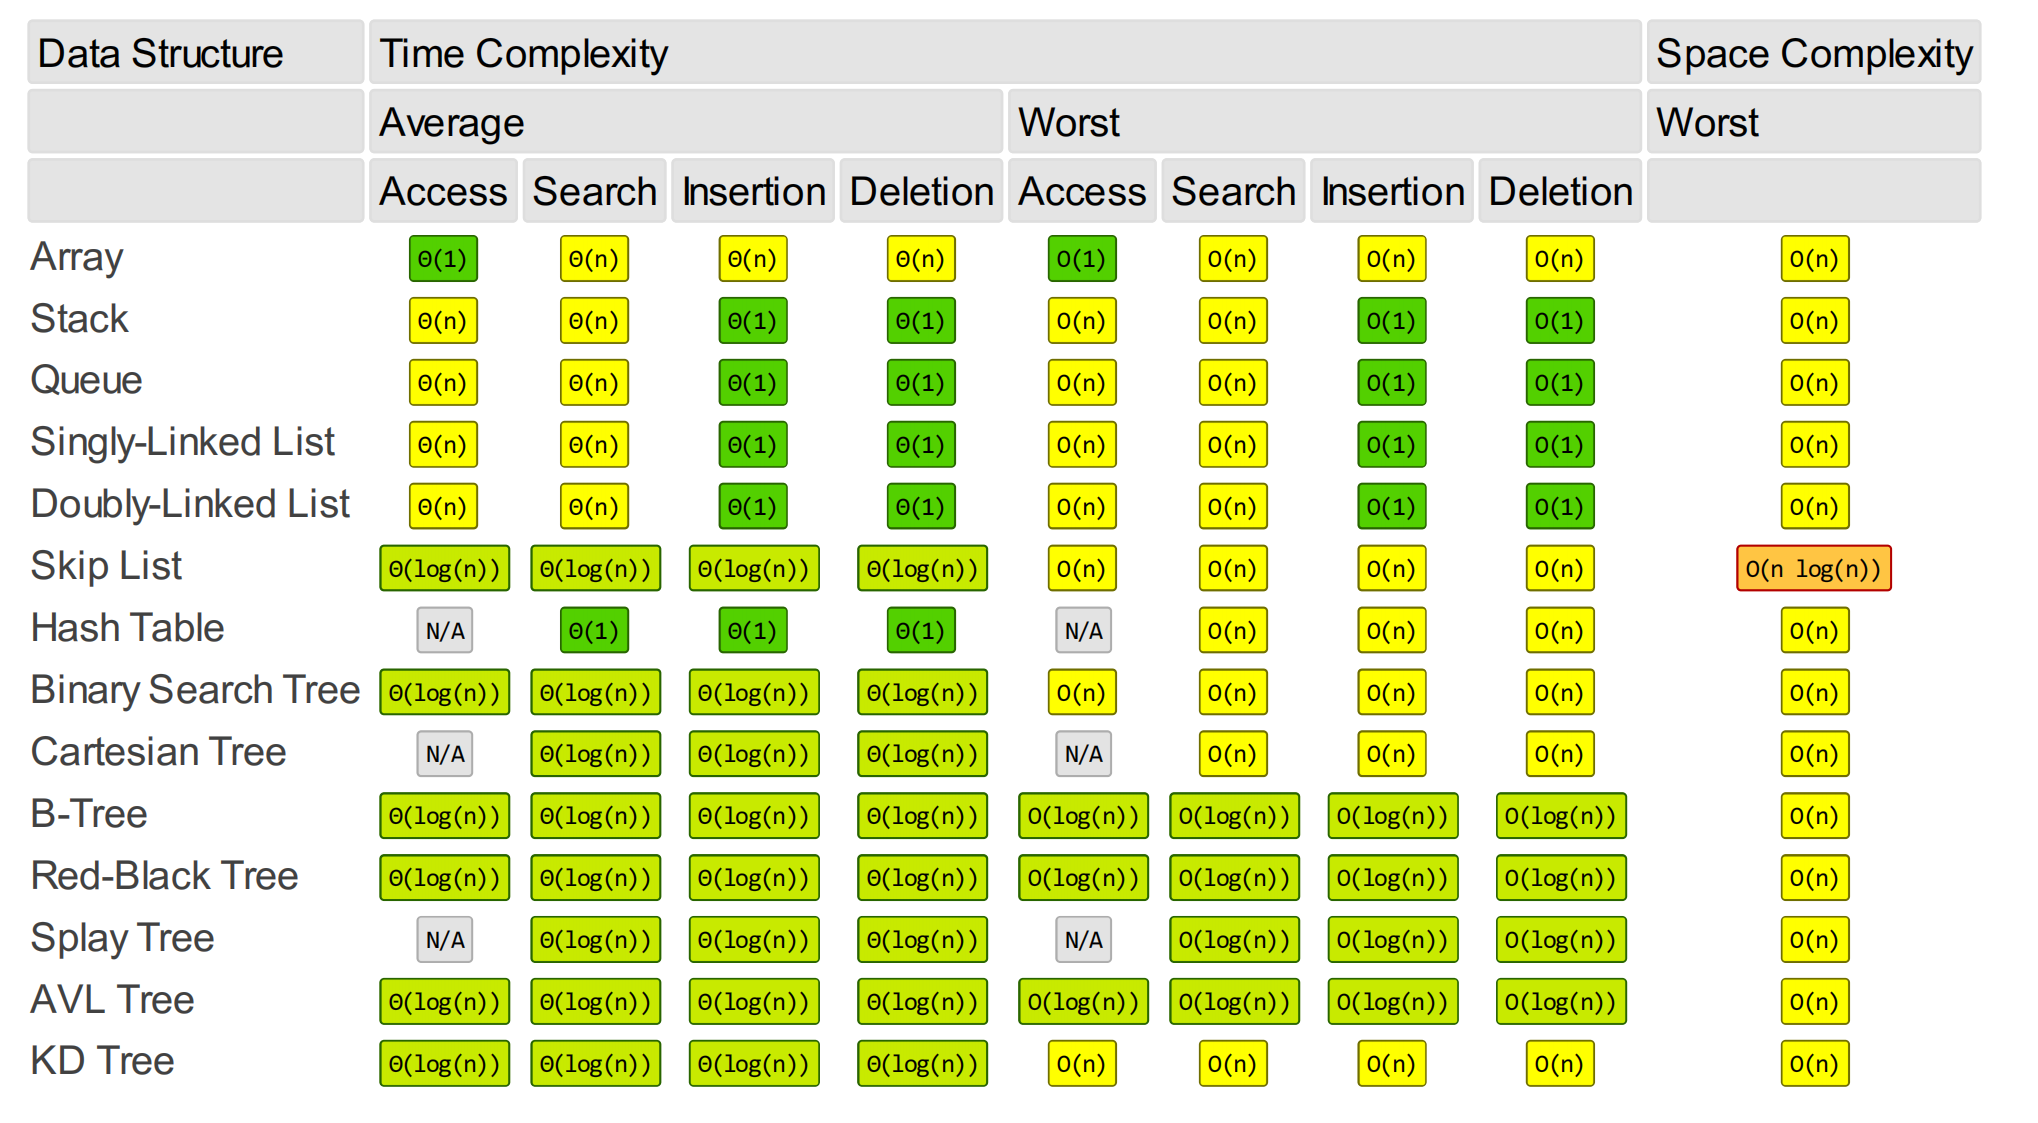
\includegraphics[width=0.9\textwidth]{images_content/1.png} %插入图片,[]中设置图片大小,{}中是图片文件名
\caption{Common Data Structure Operations} %最终文档中希望显示的图片标题
\end{figure}

\subsection{Array Sorting Algorithms}
\begin{figure}[H] %H为当前位置,!htb为忽略美学标准,htbp为浮动图形
\centering %图片居中
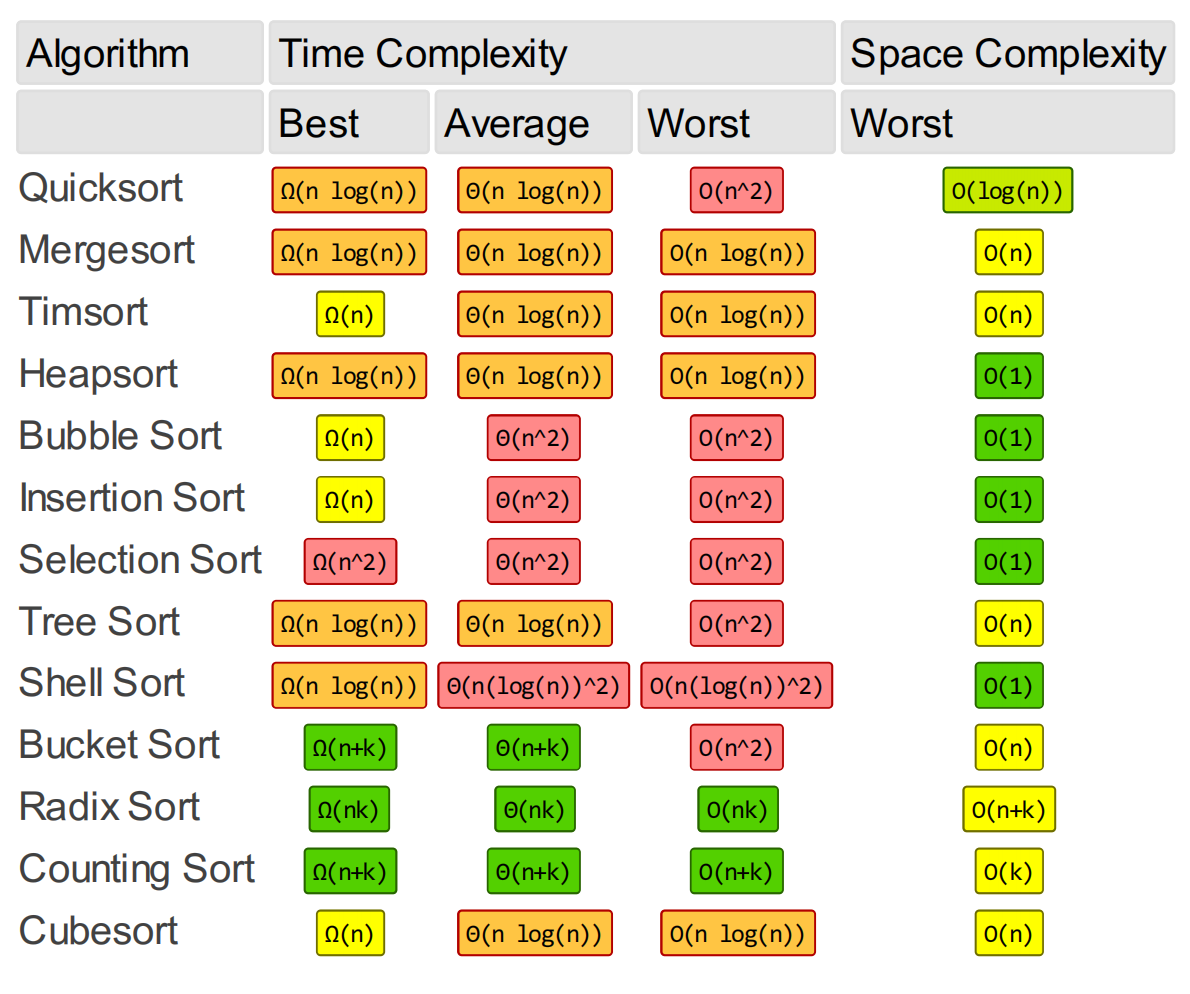
\includegraphics[width=0.7\textwidth]{images_content/2.png} %插入图片,[]中设置图片大小,{}中是图片文件名
\caption{Array Sorting Algorithms} %最终文档中希望显示的图片标题
\end{figure}

\subsection{Growth Rates}
\begin{figure}[H] %H为当前位置,!htb为忽略美学标准,htbp为浮动图形
\centering %图片居中
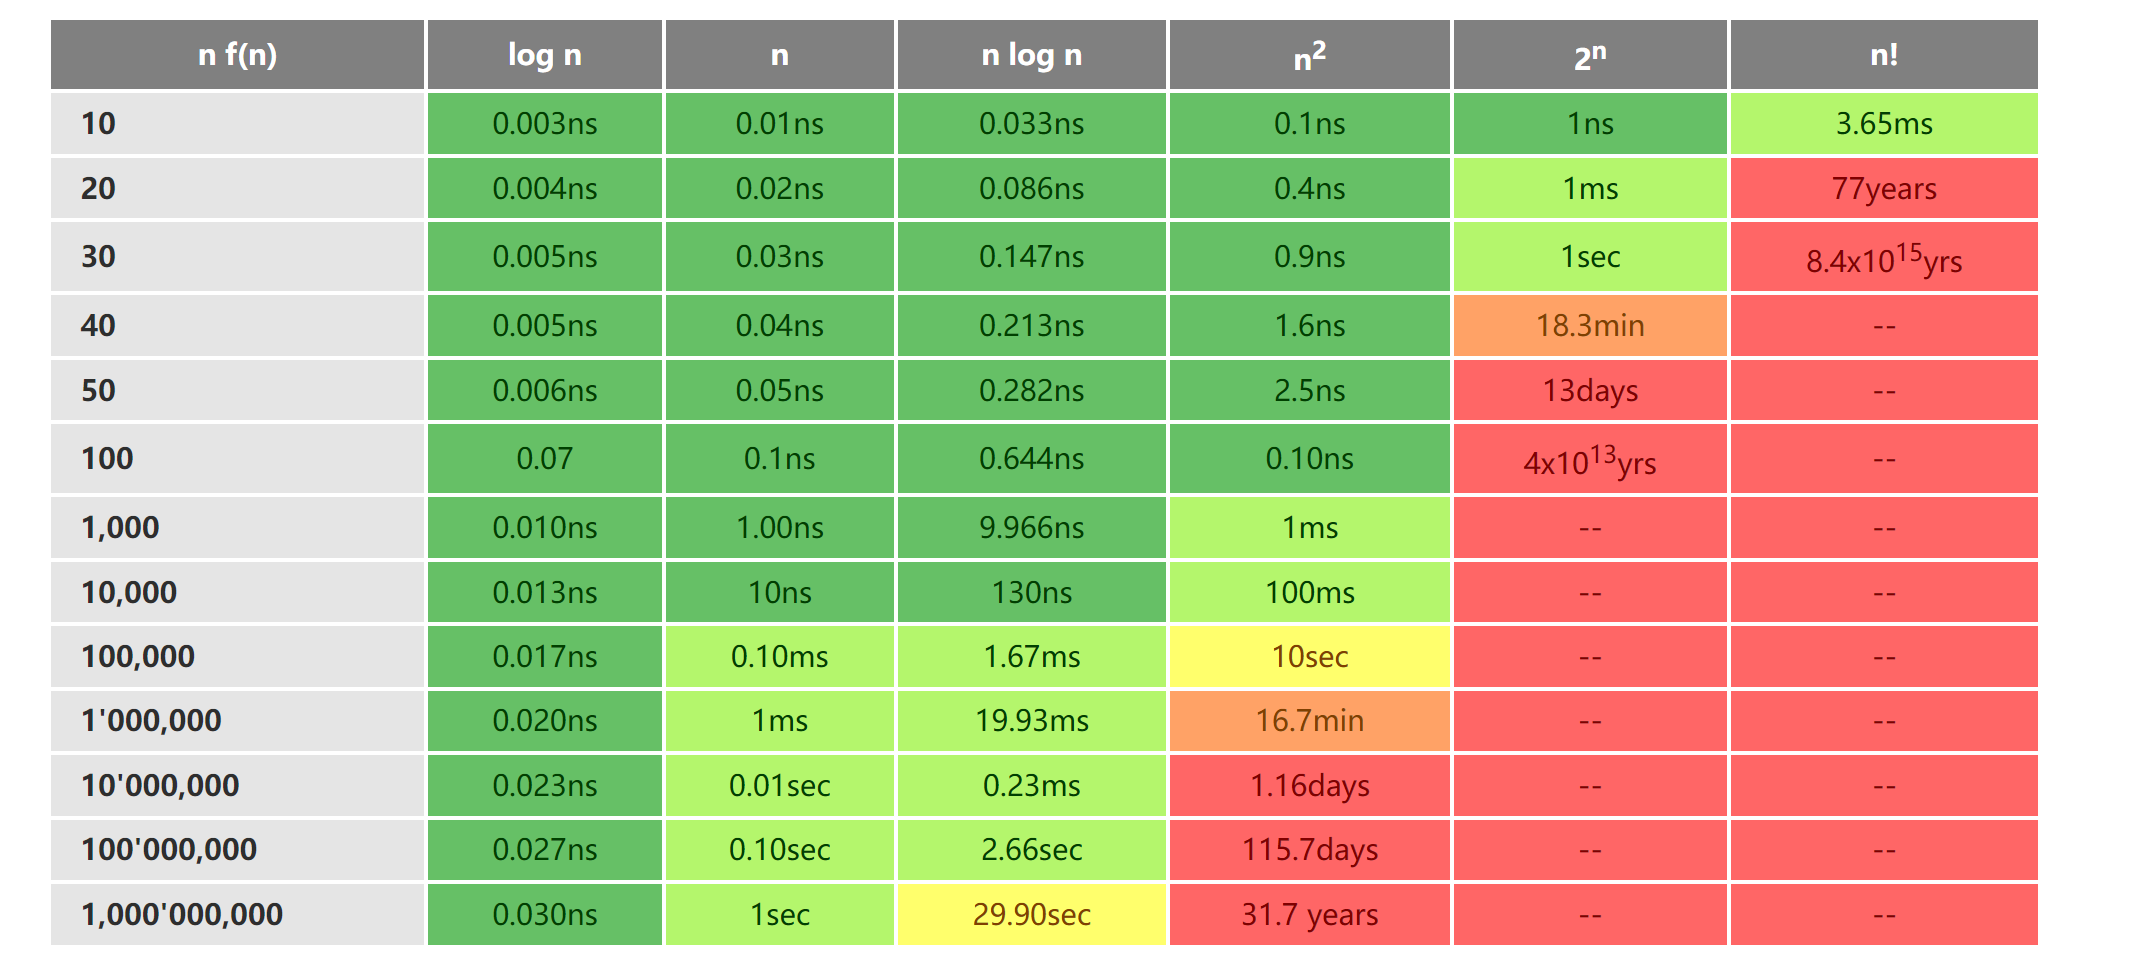
\includegraphics[width=0.9\textwidth]{images_content/3.png} %插入图片,[]中设置图片大小,{}中是图片文件名
\caption{Growth Rates} %最终文档中希望显示的图片标题
\end{figure}


\section{数据范围=>算法复杂度及算法内容}
原地址:\href{https://www.acwing.com/blog/content/32/}{https://www.acwing.com/blog/content/32/}
\begin{table}[!ht]
    \raggedleft
    \caption{由数据范围反推算法复杂度以及算法内容}
    \renewcommand\arraystretch{1.5}
    \begin{tabular}{|l|l|l|}
    \hline
        \textbf{数据范围} & \textbf{ 级别 } & \textbf{ 算法选择 } \\ \hline
        $n \le 30$ & 指数级别 & \hword{dfs+剪枝} \hword{状态压缩dp} \\ \hline
        $n \le 100$ & $O(n^3)$ & \hword{floyd} \hword{ dp } \hword{ 高斯消元 } \\ \hline
        $n \le 1000 $ & $O(n^2) O(n^2\log{n})$ & \hword{ dp } \hword{ 二分 } \hword{ 朴素版Dijkstra } \hword{ 朴素版Prim} \hword{ Bellman-Ford } \\ \hline
        $n \le 10^4$ & $O(n\sqrt{n})$  & \hword{ 块状链表 } \hword{ 分块 } \hword{ 莫队 } \\ \hline
        $n \le 10^5$ & $O(n\log{n})$ & \makecell[l]{ \hword{ 各种sort } \hword{ 线段树 } \hword{ 树状数组 } \hword{ set/map } \hword{ heap } \hword{ 拓扑排序 } \hword{ dijkstra+heap } \\ \hword{ prim+heap } \hword{ Kruskal } \hword{ spfa } \hword{ 求凸包 } \hword{ 求半平面交 } \hword{ 二分 } \hword{ CDQ分治 } \\ \hword{ 整体二分 } \hword{ 后缀数组 } \hword{ 树链剖分 } \hword{ 动态树 }} \\ \hline
        \multirow{2}*{$n \le 10^6$} & $O(n)$ & \hword{ 单调队列 } \hword{ hash } \hword{ 双指针扫描 } \hword{ 并查集 } \hword{ kmp } \hword{ AC自动机 } \\ \cline{2-3}
        & 常数较小的$O(n\log{n})$算法& \hword{ sort } \hword{ 树状数组 } \hword{ heap } \hword{ dijkstra } \hword{spfa} \\ \hline
        $n \le 10^7$  & $O(n)$ & \hword{ 双指针扫描 } \hword{ kmp } \hword{ AC自动机 } \hword{ 线性筛素数 } \\ \hline
        $n \le 10^9$ & $O(\sqrt{n})$  & \hword{ 判断质数 } \\ \hline
        $n \le 10^{18}$ & $O(\log{n})$ & \hword{ 最大公约数 } \hword{ 快速幂 } \hword{ 数位DP } \\ \hline
        $n \le 10^{1000}$ & $O((\log{n})^2)$ & \hword{ 高精度加减乘除 } \\ \hline
        $n \le 10^{100000}$ & $O(\log{k} * \log{\log{k}})$, $k$表示位数 & \hword{ 高精度加减 } \hword{ FFT/NTT } \\ \hline
    \end{tabular}
\end{table}